\section{\FVSpec:PBT$\to$FV Pipeline}
\Secl{pipeline}

We lift each PBT in the \Secr{dataset} corpus (\FVSpec:PBT) into a Lean
(\texttt{Impl.lean}, \texttt{Spec.lean}) pair (Figure~\ref{fig:pipeline},
bottom) in three phases: function discovery, agentic transpilation, and
post-production.
We call the resulting FV challenge corpus \FVSpec:FV.
 The pipeline is modeled on
FVAPPS~\cite{dougherty2025proving} but starts from PBTs rather
than programming puzzles, and adds an iterative LSP-repair loop.

\emph{Function discovery.}\label{sec:pipeline-discovery}
For each PBT we use tree-sitter to extract the function under test
(FUT) and the transitive closure of its locally-defined dependencies. For
our running example \texttt{isort}, this is just the four-line \texttt{def
isort} body itself: \texttt{insort} comes from \texttt{bisect}, which is
external and not in scope for transitive recovery. Larger PBTs in the
corpus pull in tens to hundreds of lines of internal helpers
(see Figure~\ref{fig:pbt-vs-deps}). When discovery fails---typically due
to metaclasses, decorators, or other dynamic dispatch---we emit a stub
FUT with generic type parameters so the formalization agent still
receives well-formed input.

\emph{Agentic transpilation.} A single formalization agent translates each sample, producing both
\texttt{Impl.lean} (a computable port of the FUT and its dependencies, no
\texttt{sorry}) and \texttt{Spec.lean} (one theorem per Hypothesis
assertion, with proofs left as \texttt{sorry}). This is exemplified for \texttt{isort} in 
Figure~\ref{fig:running-example}.
After each generation step we type-check the output via the Lean LSP
(over MCP) and \texttt{lake build}; on failure, the compiler diagnostics
are fed back to the agent and a revised translation is requested. The
loop terminates on success or after 16 tool-iterations.

\emph{Post-production.} We first extract LLM turn counts from the raw
\texttt{.eval} archives produced by the formalization agent, which runs
as an Inspect~AI~\cite{UKAISI_inspect_2024} task. We then
collapse runs into a single JSONL, deduplicating by sample id and
tie-breaking with a quality score (structural faithfulness, theorem
count, unit-tests, implementation success). Next, we re-run
\texttt{lake build} on each retained sample and drop failures, which we
classify into nine families: timeouts, well-founded recursion,
unknown identifiers, failures to synthesize, type mismatches, syntax
errors, missing functions, application errors, and declaration errors.
We then run \texttt{radon} on the Python source and a custom AST
analyzer on the Lean artifacts to extract line counts, theorem and
\texttt{def} counts, residual \texttt{sorry}/\texttt{admit}s, and
axioms. Finally, conditioning on these metrics, we assign a binary
easy/hard label using \texttt{claude-haiku-4-5} as judge, together with
a calibrated confidence score and a short rationale.

The structural-faithfulness score used in the merge
tie-break is a fixed weighted average of five sub-scores, each measuring
how much of a Python-side artifact survives translation:
\begin{equation}
  S = 0.25\,S_{\text{param}} + 0.25\,S_{\text{type}} + 0.20\,S_{\text{strat}} + 0.20\,S_{\text{assert}} + 0.10\,S_{\text{dep}}
  \label{eq:faithfulness}
\end{equation}
where each sub-score is in $[0,1]$: $S_{\text{param}}$ (parameter coverage), $S_{\text{type}}$ (type correspondence), $S_{\text{strat}}$ (strategy coverage), $S_{\text{assert}}$ (assertion coverage), and $S_{\text{dep}}$ (dependency coverage). For
\texttt{isort}, parameter coverage rewards the Lean theorem taking a
single \texttt{List Int} matching Python's \texttt{lst}; type
correspondence verifies that Python's \texttt{list[int]} maps to
\texttt{List Int}; strategy coverage tracks that
\texttt{st.lists(st.integers())} ranges over arbitrary integer lists,
with no missing bounds in the Lean version; assertion coverage rewards
both Python assertions producing a corresponding Lean theorem; and
dependency coverage rewards every named helper recovered in function
discovery surviving into \texttt{Impl.lean}. Sub-scores ship alongside
the overall score so consumers can re-weight or filter.

\subsection{Pipeline yield}
\label{sec:pipeline-yield}

The published \FVSpec:FV dataset contains
\textbf{9{,}415 samples} drawn from \textbf{2{,}772 distinct PBTs}
(Figure~\ref{fig:pipeline}, bottom right):
formalization succeeded for $2{,}772$ of $11{,}039$ input PBTs ($25\%$);
the rest were dropped by \texttt{lake build}. The mean sample carries 8 theorems
(median 6, max 66) and median structural faithfulness 0.65 (Figure~\ref{fig:faithfulness}). A complete Lean implementation was generated for 59\% of samples; the remaining 41\% ship
against a stub \texttt{Impl.lean}, so the theorem statement is well-typed
but the body it constrains is opaque. The Claude Haiku grader splits the
dataset 62\%/38\% hard/easy. Where a PBT yields multiple compiling
formalizations (mean 3.4 formalizations per PBT, range 1--15), all are kept; the
\texttt{is\_canonical} field marks the highest-quality version per PBT.

\begin{figure}[t]
  \centering
  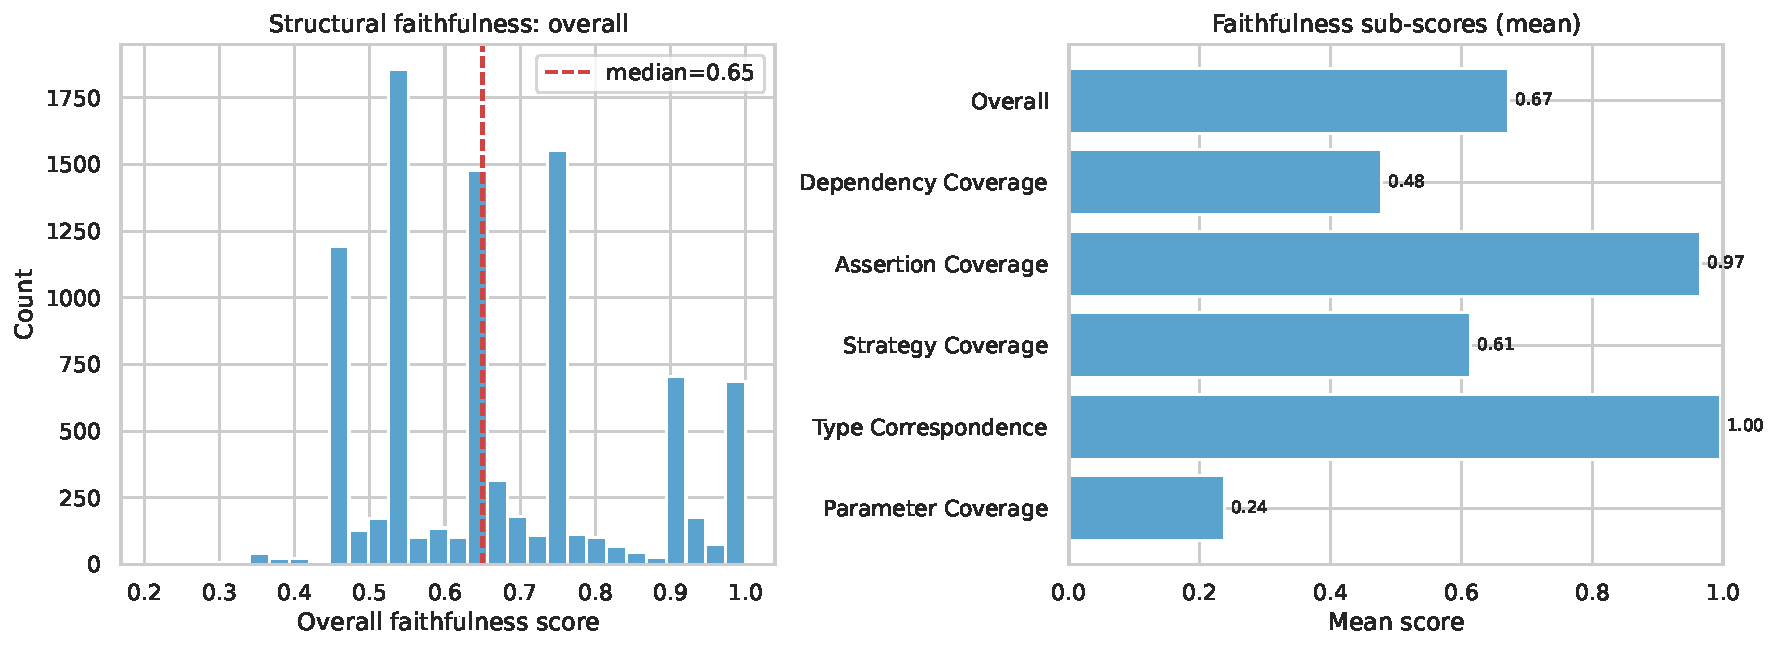
\includegraphics[width=\linewidth]{figs/structural_faithfulness.pdf}
  \caption{Structural-faithfulness scores across the published \FVSpec:FV
    dataset. \emph{Left}: histogram of per-sample overall scores
    (median 0.65; the multi-modal shape reflects the discrete denominators
    of the underlying ratios). \emph{Right}: mean per-sub-metric scores.
    Type correspondence ($1.00$) and assertion coverage ($0.97$) are
    near-saturated---most translations preserve types and predicates---while
    parameter coverage ($0.24$) and dependency coverage ($0.48$) are the
    weak links, dragging the overall mean down to $0.67$. The high
    variance in per-sample scores is exactly what the
    \texttt{is\_canonical} flag exploits when multiple formalizations
    of the same PBT are available.}
  \label{fig:faithfulness}
\end{figure}

\begin{figure}[t]
\centering
\begin{tikzpicture}[
  font=\footnotesize,
  box/.style={draw, rounded corners=2pt, fill=gray!5, inner sep=4pt, align=center,
              text width=22mm, minimum height=11mm, line width=0.4pt},
  outbox/.style={draw, rounded corners=2pt, fill=blue!8, inner sep=4pt, align=center,
              text width=22mm, minimum height=11mm, line width=0.6pt,
              font=\footnotesize\bfseries},
  arr/.style={-{Latex[length=2mm]}, gray!50!black, line width=0.5pt},
  group/.style={draw, dashed, rounded corners, inner sep=4mm,
                gray!60!black, line width=0.6pt},
  hdr/.style={font=\small\sffamily\bfseries},
  source/.style={font=\footnotesize\itshape},
  node distance=4mm and 4mm,
]
  % --- Row 1: FVSpec:PBT extraction (top) ---
  \node[source]                 (gh)    {GitHub};
  \node[box, right=8mm of gh]   (disc1) {Discovery\\\scriptsize\rmfamily 19{,}808 repos};
  \node[box, right=of disc1]    (lic)   {License filter\\\scriptsize\rmfamily copyleft~$\to$~drop};
  \node[box, right=of lic]      (ext)   {Extract\\\scriptsize\rmfamily \texttt{@given} via ripgrep};
  \node[outbox, right=of ext]   (pbtout){11{,}039 PBTs\\\scriptsize\rmfamily\mdseries 333 repos};
  \draw[arr] (gh.east) -- (disc1.west);
  \foreach \a/\b in {disc1/lic, lic/ext, ext/pbtout} \draw[arr] (\a) -- (\b);

  % --- Row 2: FVSpec:FV generation (bottom) ---
  \node[box, below=16mm of disc1] (disc2) {Function discovery\\\scriptsize\rmfamily tree-sitter};
  \node[box, right=of disc2]      (form)  {Agentic transpilation\\\scriptsize\rmfamily LSP loop, $\leq$16 iter};
  \node[box, right=of form]       (post)  {Post-production\\\scriptsize\rmfamily merge / validate};
  \node[outbox, right=of post]    (fvout) {9{,}415 samples\\\scriptsize\rmfamily\mdseries 2{,}772 PBTs};
  \foreach \a/\b in {disc2/form, form/post, post/fvout} \draw[arr] (\a) -- (\b);

  % LSP repair self-loop on the formalization agent (explicit Bezier so it actually renders)
  \draw[arr] ([xshift=-2.5mm]form.north)
        .. controls ([xshift=-2.5mm,yshift=6mm]form.north)
                and ([xshift= 2.5mm,yshift=6mm]form.north)
        .. ([xshift= 2.5mm]form.north);

  % --- Group dashed boxes (do NOT include the GitHub source label) ---
  \node[group, fit=(disc1)(pbtout)] (g1) {};
  \node[group, fit=(disc2)(fvout)]  (g2) {};

  % --- Left-aligned labels at the top-left of each dashed group ---
  \node[hdr, anchor=south west, xshift=-2cm, yshift=0.3mm] at (g1.north east) {\FVSpec:PBT};
  \node[hdr, anchor=south west, xshift=-2cm,  yshift=0.3mm] at (g2.north east) {\FVSpec:FV};

  % --- Bridge arrow: from the 11,039-PBTs output box, down past the dashed group edge, then left across the inter-group gap, then down into function discovery ---
  \draw[arr] ([xshift=-0.5cm] pbtout.south) -- ([xshift=-0.5cm,yshift=-8mm]pbtout.south) -| (disc2.north);
\end{tikzpicture}
\caption{The full \FVSpec generation pipeline (FVC = FV challenge). \emph{Top} (\FVSpec:PBT):
the input PBT corpus is scraped from public GitHub repositories
(\Secr{dataset}). \emph{Bottom} (\FVSpec:FV): each PBT is lifted into a
Lean (Impl, Spec) pair via tree-sitter--based function discovery, an
agentic transpilation step (with the LSP-repair self-loop), and a
deterministic post-production stage that validates, deduplicates, and
grades the output; 11{,}039 PBTs enter and 9{,}415 FVCs (from 2{,}772 distinct PBTs) emerge.}
\label{fig:pipeline}
\end{figure}
